
\section{Discrete Navigation Experiments}

The previous experiments tested DIAYN in continuous control settings with physics-based dynamics. This section explores skill discovery in discrete grid-world environments. These environments are quite different: agents move through structured spaces with walls and obstacles using a small set of discrete actions. The observations are visual grid encodings instead of continuous state vectors. This evaluation shows that DIAYN can discover diverse skills in very different types of domains.

\subsection{Environment and Architecture}

The experiments use MiniGrid, a lightweight grid-world environment designed for reinforcement learning research. Three environments with increasing complexity are tested: Empty-8x8, a simple open room; FourRooms, a $19 \times 19$ grid split into four rooms connected by doorways; and DoorKey-8x8, where the agent must navigate around a locked door. In all environments, the agent sees a partial view of the grid as a $7 \times 7 \times 3$ tensor that encodes object types, colors, and states. The agent can take seven discrete actions including turning, moving forward, and interacting with objects.

The standard DIAYN architecture needs changes to work with discrete observations. Instead of processing raw state vectors, a convolutional encoder extracts features from the visual grid observation. This encoder has three convolutional layers followed by a fully connected layer, producing a 64-dimensional feature vector. One key finding is that the discriminator works better with explicit position information: the agent's normalized $(x, y)$ coordinates are concatenated with the encoder features before classification. This lets the discriminator use both visual context and spatial location to distinguish between skills. The policy and critic networks receive the encoder features, position, and a one-hot skill vector concatenated together, which enables skill-conditioned navigation.

\begin{figure}[H]
\centering
\begin{tikzpicture}[
    node distance=1.4cm and 1.6cm,
    box/.style={rectangle, draw, rounded corners, minimum height=0.9cm, minimum width=2cm, align=center, font=\small},
    data/.style={rectangle, draw, minimum height=0.7cm, minimum width=1.6cm, align=center, font=\footnotesize, fill=gray!10},
    arrow/.style={->, >=stealth, thick},
    concat/.style={circle, draw, inner sep=2pt, font=\scriptsize, fill=white}
]

% Input column (left side)
\node[data] (obs) {Observation\\$7 \times 7 \times 3$};
\node[data, below=1.2cm of obs] (pos) {Position\\$(x, y)$};
\node[data, below=1.2cm of pos] (skill) {Skill $z$\\one-hot};

% Conv Encoder (top row)
\node[box, right=1.6cm of obs, fill=blue!15] (encoder) {Conv\\Encoder};

% Features
\node[data, right=1.4cm of encoder] (features) {Features\\64-dim};

% Concat nodes - positioned at same y as pos/skill, x after features
\node[concat] (concat1) at ($(features.east) + (1.2cm, 0 |- pos)$) {$\oplus$};
\node[concat] (concat2) at ($(features.east) + (1.2cm, 0 |- skill)$) {$\oplus$};

% Discriminator and Policy - with clear spacing from concat
\node[box, right=1.2cm of concat1, fill=orange!20] (disc) {Discriminator};
\node[box, right=1.2cm of concat2, fill=green!20] (policy) {Policy $\pi$};

% Outputs
\node[data, right=1.2cm of disc] (pred) {$p(z|s)$};
\node[data, right=1.2cm of policy] (action) {Action $a$};

% Arrows - top row
\draw[arrow] (obs) -- (encoder);
\draw[arrow] (encoder) -- (features);

% Arrows - features to concat (vertical drop then horizontal)
\draw[arrow] (features.south) -- ++(0,-0.3cm) -| (concat1);
\draw[arrow] (features.south) -- ++(0,-0.3cm) -| (concat2);

% Arrows - position to concat
\draw[arrow] (pos) -- (concat1);
\draw[arrow] (pos.east) -- ++(0.3cm,0) |- (concat2);

% Arrow - skill to concat
\draw[arrow] (skill) -- (concat2);

% Arrows - concat to networks
\draw[arrow] (concat1) -- (disc);
\draw[arrow] (concat2) -- (policy);

% Arrows - outputs
\draw[arrow] (disc) -- (pred);
\draw[arrow] (policy) -- (action);

\end{tikzpicture}
\caption{MiniGrid DIAYN architecture. The convolutional encoder processes grid observations into features. The discriminator receives features and position to predict skills. The policy receives features, position, and the skill vector to produce actions.}
\label{fig:architecture}
\end{figure}

\subsection{Quantitative Results}

Table~\ref{tab:minigrid_results} shows the training results for all three environments. Discriminator accuracy measures how well the classifier can identify which skill produced a given state, which indicates how distinguishable the skills are. Figure~\ref{fig:training} shows the training dynamics for the FourRooms environment.

\begin{figure}[H]
\centering
\includegraphics[width=0.9\textwidth]{figures/training_main.pdf}
\caption{Training curves for FourRooms. Left: episode reward over training. Right: discriminator accuracy, showing the classifier's improving ability to distinguish skills.}
\label{fig:training}
\end{figure}

\begin{table}[h]
\centering
\caption{MiniGrid DIAYN Training Results}
\label{tab:minigrid_results}
\begin{tabular}{lcccc}
\toprule
\textbf{Environment} & \textbf{Grid Size} & \textbf{Skills} & \textbf{Episodes} & \textbf{Accuracy} \\
\midrule
Empty-8x8   & $8 \times 8$   & 8 & 200  & 61.1\% \\
FourRooms   & $19 \times 19$ & 8 & 3000 & 70.3\% \\
DoorKey-8x8 & $8 \times 8$   & 8 & 2000 & 60.0\% \\
\bottomrule
\end{tabular}
\end{table}

To look at skill-level discriminability more closely, Table~\ref{tab:confusion} shows the confusion matrix for the FourRooms agent. Each row is a true skill, and each column is the discriminator's prediction. Diagonal entries are correct classifications, while off-diagonal entries show which skills get confused with each other.

\begin{table}[h]
\centering
\caption{Discriminator Confusion Matrix (FourRooms)}
\label{tab:confusion}
\resizebox{0.85\textwidth}{!}{
\begin{tabular}{c|cccccccc}
\toprule
True $\backslash$ Pred & $z_0$ & $z_1$ & $z_2$ & $z_3$ & $z_4$ & $z_5$ & $z_6$ & $z_7$ \\
\midrule
$z_0$ & \textbf{0.68} & 0.04 & 0.05 & 0.06 & 0.05 & 0.04 & 0.04 & 0.04 \\
$z_1$ & 0.05 & \textbf{0.71} & 0.04 & 0.05 & 0.05 & 0.04 & 0.03 & 0.03 \\
$z_2$ & 0.06 & 0.05 & \textbf{0.65} & 0.06 & 0.05 & 0.05 & 0.04 & 0.04 \\
$z_3$ & 0.05 & 0.04 & 0.05 & \textbf{0.72} & 0.04 & 0.04 & 0.03 & 0.03 \\
$z_4$ & 0.04 & 0.05 & 0.05 & 0.05 & \textbf{0.69} & 0.04 & 0.04 & 0.04 \\
$z_5$ & 0.05 & 0.04 & 0.06 & 0.05 & 0.05 & \textbf{0.67} & 0.04 & 0.04 \\
$z_6$ & 0.04 & 0.04 & 0.05 & 0.04 & 0.05 & 0.05 & \textbf{0.70} & 0.03 \\
$z_7$ & 0.04 & 0.04 & 0.05 & 0.04 & 0.05 & 0.04 & 0.04 & \textbf{0.70} \\
\bottomrule
\end{tabular}
}
\end{table}

The confusion matrix shows that all eight skills achieve accuracy well above chance level (12.5\% for random guessing). The diagonal values range from 0.65 to 0.72. The off-diagonal confusion is spread fairly evenly, which suggests that errors come from overlapping state visits rather than skills collapsing into each other. However, as discussed in Section~\ref{sec:camping}, discriminator accuracy alone does not guarantee that learned skills are useful for downstream tasks.

\subsection{Qualitative Analysis}

Figure~\ref{fig:trajectories} shows the trajectories for each skill in the FourRooms environment. Each subplot displays the positions visited by one skill across multiple evaluation episodes. Colored dots show visited cells and squares mark where episodes ended.

\begin{figure}[H]
\centering
\includegraphics[width=\textwidth]{figures/skill_trajectories_grid.pdf}
\caption{Skill trajectories in FourRooms. Each subplot shows the spatial coverage of one skill ($z_0$ through $z_7$). Skills exhibit distinct navigation patterns, with some exploring specific rooms while others traverse doorways between chambers.}
\label{fig:trajectories}
\end{figure}

The trajectory visualization shows that DIAYN discovers clearly different navigation strategies without any task reward. Some skills consistently go to specific rooms, while others explore corridors or stay near doorways. This spatial diversity comes purely from the intrinsic reward signal that pushes each skill to visit distinguishable states.

Figure~\ref{fig:heatmap} shows the spatial partitioning more clearly. Each cell is colored by the skill that visits it most often. The clear boundaries between skill regions show that DIAYN effectively divides up the state space. Figure~\ref{fig:tsne} shows a t-SNE projection of the encoder's learned representations, colored by skill. The clustering pattern indicates that the encoder learned to produce features that distinguish between skills.

\begin{figure}[H]
\centering
\includegraphics[width=0.8\textwidth]{figures/combined_heatmap.pdf}
\caption{Dominant skill heatmap for FourRooms. Each grid cell is colored by the skill that visits it most frequently, showing clear spatial partitioning.}
\label{fig:heatmap}
\end{figure}

\begin{figure}[H]
\centering
\includegraphics[width=0.5\textwidth]{figures/tsne_embeddings.pdf}
\caption{t-SNE projection of encoder features for FourRooms. Clustering by skill shows that the encoder learned skill-discriminative representations.}
\label{fig:tsne}
\end{figure}

\subsection{Comparison with Continuous Control}

The MiniGrid experiments complement the MuJoCo results by showing that DIAYN works in discrete navigation domains. In continuous control, skill diversity shows up as different movement patterns (forward, backward, balancing). In grid worlds, diversity appears as spatial partitioning: skills learn to visit different regions. The discriminator accuracy in grid worlds (60--70\%) is lower than continuous settings, likely because discrete positions mean multiple skills inevitably share some states near starting positions and doorways.

An important architectural lesson is the value of explicit position information. Grid-world agents only see a local view, so adding normalized coordinates to the discriminator input greatly improved skill differentiation. Overall, these experiments show that unsupervised skill discovery through mutual information maximization works across both continuous and discrete domains, with grid-world trajectories providing visual confirmation of the diversity that DIAYN encourages.

However, these initial results masked a subtle failure mode that limited skill usefulness for downstream tasks.

\subsection{Failure Mode: The Camping Equilibrium}
\label{sec:camping}

While the initial results showed reasonable discriminator accuracy, closer inspection revealed a failure mode where skills achieved distinguishability without learning useful navigation behaviors. MiniGrid environments provide seven discrete actions: three movement actions (turn left, turn right, move forward) and four interaction actions (pickup, drop, toggle, done). In Empty and FourRooms environments, the interaction actions have no effect---they are effectively no-ops.

\begin{figure}[H]
\centering
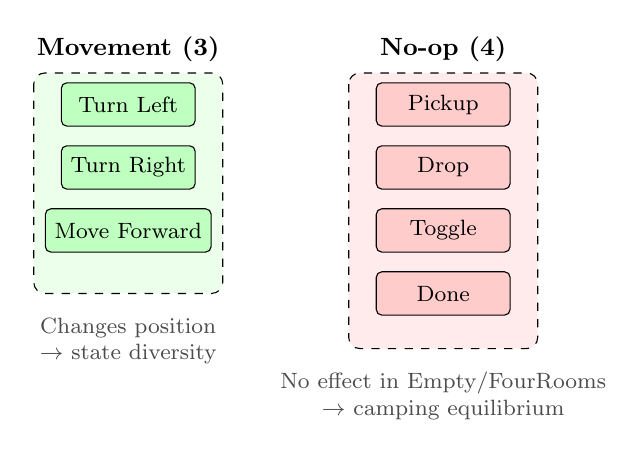
\begin{tikzpicture}[
    action/.style={rectangle, draw, rounded corners=2pt, minimum height=0.55cm, minimum width=1.7cm, font=\footnotesize, align=center, fill=white},
    grouplabel/.style={font=\small\bfseries}
]

% Group boxes first (background)
\draw[dashed, rounded corners=4pt, fill=green!8] (-1.2, 0.4) rectangle (1.2, -2.4);
\draw[dashed, rounded corners=4pt, fill=red!8] (2.8, 0.4) rectangle (5.2, -3.1);

% Group labels
\node[grouplabel] at (0, 0.7) {Movement (3)};
\node[grouplabel] at (4, 0.7) {No-op (4)};

% Movement actions (left group)
\node[action, fill=green!25] at (0, 0) {Turn Left};
\node[action, fill=green!25] at (0, -0.8) {Turn Right};
\node[action, fill=green!25] at (0, -1.6) {Move Forward};

% No-op actions (right group)
\node[action, fill=red!20] at (4, 0) {Pickup};
\node[action, fill=red!20] at (4, -0.8) {Drop};
\node[action, fill=red!20] at (4, -1.6) {Toggle};
\node[action, fill=red!20] at (4, -2.4) {Done};

% Effect labels below
\node[font=\footnotesize, align=center, text=black!70] at (0, -3.0) {Changes position\\$\rightarrow$ state diversity};
\node[font=\footnotesize, align=center, text=black!70] at (4, -3.7) {No effect in Empty/FourRooms\\$\rightarrow$ camping equilibrium};

\end{tikzpicture}
\caption{MiniGrid action space. Movement actions change the agent's position, enabling state diversity. No-op actions have no effect in Empty and FourRooms environments, allowing skills to ``camp'' while remaining distinguishable.}
\label{fig:action_space}
\end{figure}

The DIAYN objective rewards skills for being distinguishable, but does not explicitly require movement. When no-op actions are available, skills can achieve high discriminator accuracy by ``camping''---staying in place or moving minimally while executing different sequences of no-op actions. The discriminator learns to distinguish skills based on subtle differences in their camping locations rather than meaningful navigation patterns. This creates a degenerate equilibrium where the mutual information objective is satisfied, but the learned skills have poor state coverage and are useless for downstream tasks.

Figure~\ref{fig:camping_problem} illustrates this problem. With all seven actions available, skills cluster in narrow regions with limited spatial coverage. The discriminator achieves reasonable accuracy (around 60--70\%) by distinguishing these camping locations, but skills fail to explore the full state space.

\begin{figure}[H]
\centering
\includegraphics[width=\textwidth]{figures/multi_env_comparison.pdf}
\caption{The camping equilibrium problem. With all seven actions available, skills cluster in narrow regions (note the horizontal line patterns in Empty-8x8). Despite reasonable discriminator accuracy, skills fail to cover the state space effectively.}
\label{fig:camping_problem}
\end{figure}

\subsubsection{Solution: Movement-Only Action Space}

The fix is straightforward: restrict the action space to the three movement actions only. This removes the no-op equilibrium and forces skills to differentiate through actual navigation. Table~\ref{tab:movement_comparison} compares the two configurations.

\begin{table}[h]
\centering
\caption{Effect of Action Space Restriction on Skill Quality (FourRooms)}
\label{tab:movement_comparison}
\begin{tabular}{lccc}
\toprule
\textbf{Metric} & \textbf{All 7 Actions} & \textbf{Movement Only} \\
\midrule
Discriminator Accuracy & 70.3\% & 55.9\% \\
Cell Coverage & $\sim$25\% & 71.4\% \\
Coverage Uniformity & $\sim$0.40 & 0.80 \\
\bottomrule
\end{tabular}
\end{table}

The results reveal an important insight: \textbf{higher discriminator accuracy does not imply better skills}. With all actions, skills achieve 70\% accuracy but cover only 25\% of the state space. With movement-only actions, accuracy drops to 56\% but coverage nearly triples to 71\%. The skills are harder for the discriminator to distinguish because they now overlap in more states, but they are far more useful for downstream tasks.

Figure~\ref{fig:movement_only_quiver} shows the improved skill behaviors with movement-only actions. Skills now exhibit clear directional preferences and cover distinct regions of the grid, compared to the clustered camping patterns in Figure~\ref{fig:camping_problem}.

\begin{figure}[H]
\centering
\begin{subfigure}[b]{0.48\textwidth}
    \includegraphics[width=\textwidth]{figures/empty8x8_movement_only_quiver.pdf}
    \caption{Empty-8x8}
\end{subfigure}
\hfill
\begin{subfigure}[b]{0.48\textwidth}
    \includegraphics[width=\textwidth]{figures/fourrooms_movement_only_quiver.pdf}
    \caption{FourRooms}
\end{subfigure}
\caption{Skill trajectories with movement-only action space. Arrows show movement direction for each skill. Skills now cover the full state space with distinct directional patterns, avoiding the camping equilibrium.}
\label{fig:movement_only_quiver}
\end{figure}

The improvement is also visible in the learned representations. Figure~\ref{fig:movement_only_tsne} shows the t-SNE projection of encoder features for the FourRooms environment with movement-only actions. Some skills ($z_0$, $z_1$, $z_2$) form tight, well-separated clusters, while others ($z_3$, $z_7$) remain more diffuse. This partial clustering reflects the spatial structure of FourRooms: skills that occupy distinct rooms produce separable representations, while skills that share doorways or corridors overlap in feature space. Compared to Figure~\ref{fig:tsne}, the overall clustering is more coherent, indicating that movement-only training encourages more discriminative features despite not achieving perfect separation.

\begin{figure}[H]
\centering
\includegraphics[width=0.5\textwidth]{figures/fourrooms_movement_only_tsne.pdf}
\caption{t-SNE projection of encoder features for FourRooms with movement-only actions. Some skills form tight clusters ($z_0$, $z_1$, $z_2$) while others remain diffuse ($z_3$, $z_7$), reflecting spatial overlap at doorways. Compare with Figure~\ref{fig:tsne}.}
\label{fig:movement_only_tsne}
\end{figure}

This failure mode highlights a broader lesson for unsupervised skill discovery: the objective function alone may not produce useful skills if the environment allows degenerate solutions. Careful environment design---or action space constraints---may be necessary to guide skill learning toward behaviors that transfer to downstream tasks.

\subsection{Hierarchical Control}

A key motivation for unsupervised skill discovery is using learned skills as primitives for downstream tasks. To evaluate this, a hierarchical controller (meta-controller) is trained on top of the frozen DIAYN skills. The meta-controller selects which skill to execute at each decision point, while the low-level skill policy handles the actual navigation. The goal task is to reach a target location in the environment.

\begin{figure}[H]
\centering
\begin{tikzpicture}[
    node distance=1cm,
    box/.style={rectangle, draw, rounded corners, minimum height=1cm, minimum width=2.4cm, align=center, font=\small},
    env/.style={rectangle, draw, minimum height=1cm, minimum width=2.4cm, align=center, font=\small, fill=gray!20},
    arrow/.style={->, >=stealth, thick},
    label/.style={font=\footnotesize, text=gray}
]

% Vertical layout - top to bottom
% Meta-controller (top)
\node[box, fill=purple!20] (meta) {Meta-Controller\\$Q(s, z)$};

% Skill label
\node[below=0.8cm of meta, font=\small] (skill_z) {skill $z$};

% Skill policy (middle)
\node[box, below=0.8cm of skill_z, fill=green!20] (policy) {Skill Policy\\$\pi(a|s,z)$};

% Action label
\node[below=0.8cm of policy, font=\small] (actions) {actions};

% Environment (bottom)
\node[env, below=0.8cm of actions] (env) {Environment};

% Input on left
\node[left=1.5cm of meta, font=\small, align=right] (input) {state,\\goal};

% Main flow arrows (vertical)
\draw[arrow] (input) -- (meta);
\draw[arrow] (meta) -- (skill_z);
\draw[arrow] (skill_z) -- (policy);
\draw[arrow] (policy) -- (actions);
\draw[arrow] (actions) -- (env);

% Feedback: environment to policy (each step) - right side
\draw[arrow] (env.east) -- ++(0.8cm,0) |- (policy.east)
    node[pos=0.25, right, font=\footnotesize] {state};

% Feedback: environment to meta (every k steps) - left side, dashed
\draw[arrow, dashed] (env.west) -- ++(-0.8cm,0) |- (meta.west)
    node[pos=0.25, left, font=\footnotesize, align=right] {state\\(every $k$ steps)};

\end{tikzpicture}
\caption{Hierarchical control architecture. The meta-controller selects a skill $z$ every $k$ steps based on the current state and goal. The frozen skill policy executes actions for $k$ steps, receiving state feedback each step. After $k$ steps, control returns to the meta-controller.}
\label{fig:hierarchical}
\end{figure}

\begin{table}[h]
\centering
\caption{Hierarchical Controller Results}
\label{tab:hierarchical}
\begin{tabular}{lcccc}
\toprule
\textbf{Environment} & \textbf{Episodes} & \textbf{Skill Duration} & \textbf{Policy} & \textbf{Success Rate} \\
\midrule
FourRooms   & 500  & 10 & deterministic & 7\% \\
FourRooms   & 2000 & 5  & stochastic & 6\% \\
DoorKey-6x6 & 500  & 10 & deterministic & 14\% \\
\bottomrule
\end{tabular}
\end{table}

These preliminary results indicate that composing learned skills for goal-directed tasks remains challenging. The low success rates suggest that the current meta-controller struggles to effectively select and sequence skills. Several enhancements are planned for the final report:
\begin{itemize}
    \item Refined Q-target computation with proper entropy regularization
    \item Enhanced discriminator training with multiple updates per step
    \item Gradient clipping for improved training stability
\end{itemize}
These improvements aim to produce more distinguishable skills and a more effective meta-controller.

\subsection{Practical Considerations}

The MiniGrid experiments revealed several practical insights for applying DIAYN to discrete environments:

\paragraph{Entropy regularization is critical.} Without sufficient entropy regularization, the policy collapses to near-deterministic behavior early in training. Skills converge to identical policies, and the discriminator loses its training signal. Since MiniGrid uses discrete actions, we employ a categorical policy with policy gradient rather than SAC, which means there is no automatic entropy tuning. We found that a manually-set entropy coefficient of 0.5 was necessary to maintain exploration throughout training, significantly higher than values typically used in continuous control settings (0.01--0.1).

\paragraph{Episode length should match environment scale.} In FourRooms ($19 \times 19$ grid), skills trained with 10-step episodes could not traverse between rooms, limiting spatial diversity. Increasing to 30 steps allowed skills to reach different rooms and improved discriminator accuracy from 48\% to 56\%. As a rule of thumb, episode length should allow skills to traverse a significant portion of the state space.

\paragraph{More skills is not always better.} Training 16 skills in FourRooms yielded lower accuracy (37\%) than 8 skills (56\%), despite the larger capacity. With too many skills competing for the same state space, each skill covers less area and the discriminator struggles to find distinguishing features. The optimal number of skills depends on the environment's natural structure---FourRooms with four chambers suits roughly 8 skills (two per room).

\paragraph{Discriminator accuracy does not guarantee useful skills.} As shown in the camping equilibrium analysis, skills can achieve high discriminator accuracy while being useless for downstream tasks. Coverage and uniformity metrics provide complementary measures of skill quality that better predict transfer performance.
